\chapter{Asking Calabasas Millionaires How They Got RICH!}

This chapter is not a blackboard lecture in the usual sense. The mathematics is commercial rather than physical: the host repeatedly asks what business a person is in, what scale that business has reached, what changed the trajectory, and what rule survives after the anecdote has been stripped away. We therefore proceed as one would in a serious set of notes. We separate unlike quantities, we keep the interviews in the order in which they appear, and we formalize only what the transcript genuinely supports.

\section{Opening Montage and the Interview Machine}

The lecture begins with a montage of supercars, occupations, and large numbers. Its function is not merely theatrical. It teaches us the recurring procedure by which the host will work: first identify the field, then identify the scale, then locate the discontinuity, and finally extract a rule. Los Angeles, from Calabasas to Malibu, is presented as a live laboratory in which that procedure can be repeated on several independent cases.

\begin{definition}
We write \(A_{\mathrm{UM}}\) for assets under management, \(R_{\mathrm{top}}\) for top-line revenue, and \(Y_{\max}\) for a best single-year figure when the transcript gives a large number without finer accounting language.
\end{definition}

The anchored quantities that later matter are the following:
\begin{align}
A_{\mathrm{UM}} &\approx 2.5\times 10^9 \,\mathrm{USD},\\
Y_{\mathrm{fashion},\max} &= 3.0\times 10^7 \,\mathrm{USD},\\
Y_{\mathrm{jewelry},\max} &= 3.5\times 10^7 \,\mathrm{USD},\\
R_{\mathrm{software},\mathrm{top}} &> 4\times 10^6 \,\mathrm{USD},\\
Y_{\mathrm{plastic},\max} &> 10^7 \,\mathrm{USD}.
\end{align}

\begin{remark}
These are not the same object. The first line is assets under management, the fourth is top-line revenue, and the remaining figures are best-year amounts reported more loosely. The chapter must not collapse them into a fake common metric.
\end{remark}

Since no validated screenshots survive for this lecture, the only legitimate figure here is an editorial schematic of the repeated interview machine:

\begin{figure}
\begin{center}
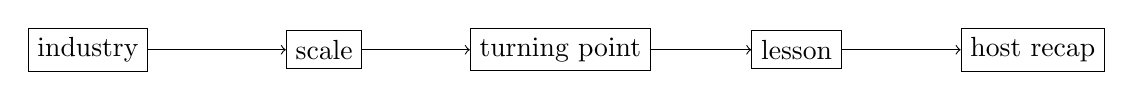
\begin{tikzpicture}
\node[draw, rectangle] (a) at (0,0) {industry};
\node[draw, rectangle] (b) at (3.0,0) {scale};
\node[draw, rectangle] (c) at (6.0,0) {turning point};
\node[draw, rectangle] (d) at (9.0,0) {lesson};
\node[draw, rectangle] (e) at (12.0,0) {host recap};
\draw[->] (a)--(b);
\draw[->] (b)--(c);
\draw[->] (c)--(d);
\draw[->] (d)--(e);
\end{tikzpicture}
\end{center}
\end{figure}

We should keep that machine in mind, because the lecture is built out of repetitions of it. Each repetition is a new case, but the logical form stays remarkably stable.

\section{Speed Under Shock: Fashion Manufacturing in COVID}

The first complete case is a manufacturer who had moved from oil and gas into fashion manufacturing. The host asks for the biggest year, receives the answer ``30 million dollars,'' and then immediately asks the only question that matters: what happened that year? The answer is that COVID hit, the factory was switched into gowns and masks, and the interviewee claims to have been the only factory in Los Angeles making them at that moment.

A compact way to organize the logic is
\begin{equation}
O \propto K\,v\,\sigma,
\end{equation}
where \(O\) is the opportunity payoff, \(K\) is the productive capability already in hand, \(v\) is the speed of the pivot, and \(\sigma\) is scarcity in the market.

The point is not that the entrepreneur found a mysterious industry. The point is that an existing productive apparatus was repurposed quickly enough to meet a temporarily undersupplied demand. The lecture is very clear on this sequence. We do not begin with invention from nothing; we begin with reconfiguration under pressure.

\subsection{Question \& Answer}

\paragraph{Question.} Why can the small entrepreneur win when a sudden market shock hits?

\paragraph{Answer.} Because the decisive variable is not size but response time. The interviewee states the principle explicitly: the small entrepreneur is dynamic and can change quickly, whereas the larger corporation may take years to catch up. In the notation above, the temporary window is captured by a large \(v\) and a still-large \(\sigma\). Once the larger firms arrive, scarcity falls and the window closes.

The host then turns the single successful year into a general lesson. The story is not merely that COVID created demand. It is that speed converts demand into profit only for those who can reorganize operations before the market normalizes.

\section{Equity, Control, and the Cost of Selling Too Early}

The same interview then pivots from shock profit to long-run ownership. This is a crucial transition. Making money in one year is one problem; retaining the structure that lets wealth compound is another. The interviewee says, in effect, that he sold a company too early, was happy with the cash, and later watched that company end up on Nasdaq.

A useful formal summary is
\begin{equation}
W_{\mathrm{retained}} \propto E\,\Gamma,
\end{equation}
where \(E\) is equity retained and \(\Gamma\) is control retained.

This is not offered as an iron law of corporate finance; it is the distilled lesson of the interview. We are told not to rush into venture capital or other outside money at the initial stage if the price is loss of control. Shares may be given out when necessary, but the controlling logic is clear: preserve enough ownership and enough decision power that later upside remains yours.

The host's recap is important here. He does not leave the point at the level of biography. He translates it into a rule for entrepreneurs starting now: early liquidity can be far smaller than the value of long-duration control. In that sense, the lecture moves from event-driven wealth to capital-structure discipline.

\section{Law, Real Estate, and Diversification Within One Competence}

The next interview begins with a surprisingly sharp answer to a broad entrepreneurial question: ``Go to law school.'' The interviewee did not become a lawyer, but he insists that legal training teaches a style of thinking and that law is deeply entangled with everything done in real estate. We are also given the scale of the business,
\begin{equation}
A_{\mathrm{UM}} \approx 2.5\times 10^9 \,\mathrm{USD}.
\end{equation}

At this point the lecture changes emphasis. The fashion case was about speed under shock. The real-estate case is about structure, analysis, and durability. The point is not simply that real estate is lucrative. The point is that a very large business may still rest on disciplined attention to contracts, regulation, and legal form.

\subsection{Question \& Answer}

\paragraph{Question.} How do we diversify without losing the advantages of specialization?

\paragraph{Answer.} The interviewee's answer is to diversify \emph{within} one area of expertise. We do not abandon the field; we vary the expression of the field. In the language of a simple schematic,
\begin{equation}
D_{\mathrm{within}} = f(T,S,G),
\end{equation}
where \(T\) denotes property type, \(S\) denotes asset size, and \(G\) denotes geography.

This is exactly how the interview unfolds. The host presses on the tension between ``get really good at one thing'' and ``diversify.'' The resolution is that commercial versus residential, large residential versus small, and one state versus another are all variations inside the same competence set. We may therefore broaden exposure without dissolving expertise.

The lecture does something else worth preserving here. It lets the strange answer, ``go to law school,'' survive long enough to become intelligible. The surprise is pedagogical. First we hear the claim; only then are we shown why the claim is not a slogan but a view about how business reality is structured.

\section{High-Ticket Craft and the Refusal To Be Average}

The plastic-surgery segment changes the type of mechanism once again. Here the business is neither an opportunistic shock pivot nor a legal-asset machine. It is a high-ticket craft business in a crowded prestige market. The interviewee reports a best year north of seven figures, says that he hit seven figures even in his first year, and explains that he entered the field not to be another practitioner in the crowd but to be the best of the best.

The important movement in this section is rhetorical. The host notices the Lamborghini and asks for final advice about owning such a car. The answer demotes the car from cause to effect. The machine is the person, not the vehicle. The car is described as a reflection of hard work rather than a mechanism of income.

What should survive into the notes is not a cult of luxury, but a business principle: in a high-ticket field, generic presence is weak. Positioning, obsessive practice, and differentiation matter. The lecture does not formalize that claim, but it states it with unusual directness. One does not merely enter a premium market; one must make oneself visibly non-ordinary inside it.

\section{Manufacturing Margin Arithmetic and Operational Leverage}

We now reach the most nearly algebraic interview in the lecture. The jewelry manufacturer reports a best year of 35 million dollars and is asked what carried the business from seven to eight figures. His answer has two parts. First, the firm stayed current on manufacturing techniques and mechanized much of the process. Second, the real business was not selling diamonds or gold; it was selling labor.

Let us write
\begin{align}
\Pi &= R - C,\\
C &= C_{\mathrm{materials}} + C_{\mathrm{labor}} + C_{\mathrm{overhead}}.
\end{align}

\begin{proposition}
If the customer already knows the market prices of the main material inputs, then the durable margin available to the manufacturer lies primarily in labor spread rather than in hidden markups on those inputs.
\end{proposition}

\begin{proof}
\begin{enumerate}
\item The interviewee states that customers know the price of diamonds.
\item He also states that customers know the price of gold because it is quoted in the market every day.
\item Those material costs therefore behave, from the customer's point of view, like transparent pass-throughs.
\item He then says that the business sold labor and nothing else.
\item Hence the main adjustable term is the difference between what the customer will pay for labor and what labor costs internally.
\end{enumerate}
Therefore we are led to the approximation
\begin{equation}
\Pi_{\mathrm{jewelry}} \approx P_{\mathrm{labor,customer}} - C_{\mathrm{labor,internal}}.
\end{equation}
\end{proof}

The second part of the argument is operational leverage. If automation and mechanization reduce internal labor cost while the customer-facing labor price does not fall one-for-one, profit rises:
\begin{equation}
\Delta \Pi_{\mathrm{jewelry}} > 0 \qquad \text{whenever} \qquad \Delta C_{\mathrm{labor,internal}} < 0.
\end{equation}

\paragraph{Worked example.} Suppose, purely for illustration, that a customer will effectively pay \(100\) dollars of labor on a piece, while internal labor cost falls from \(70\) dollars to \(55\) dollars after mechanization. Then the labor spread rises from \(30\) dollars to \(45\) dollars per unit. That is a \(50\%\) increase in per-unit margin without any change in the market prices of diamonds or gold. The numbers in this example are illustrative, but the logic is exactly the one the interview is urging on us.

\subsection{Question \& Answer}

\paragraph{Question.} If the customer already sees the prices of diamonds and gold, where does the manufacturer actually make money?

\paragraph{Answer.} In labor, and more precisely in the spread between the labor price the customer accepts and the internal labor cost the manufacturer bears. The interviewee's operational program follows immediately: stay current on technique, automate where possible, and compress internal cost without surrendering the market's willingness to pay for finished work.

The advice that follows---pay yourself first, make the money work for you, reinvest in the field you know, and keep integrity intact---should be read as a moral and capital-allocation extension of the same argument. First create a machine that throws off spread; then recycle the gains intelligently rather than leaking them into fields you do not understand.

\section{Youth, Concentration, and Long Hours}

The final interview belongs to a 22-year-old software founder running a team of about 30 people and expecting top-line revenue above four million dollars in the current year:
\begin{equation}
R_{\mathrm{software},\mathrm{top}} > 4\times 10^6 \,\mathrm{USD}.
\end{equation}

The host again asks for the mechanism, and again the answer is not merely an industry label. The founder says that when one is young, one should put one's eggs in one basket, double down, and work long hours rather than diversify too early into a retirement-style portfolio mentality. He adds that the same standard is used in judging partners and potential employees.

\begin{remark}
The lecture does not prove that concentration always dominates diversification. What it gives us is a phase-specific rule: early in the game, concentration plus time intensity may dominate breadth.
\end{remark}

Placed at the end of the chapter, this has a useful structural effect. The older interviewees stressed control, diversification within competence, and capital retention. The younger founder stresses concentration, hours, and rate of execution. The lecture ends, then, not with a universal theorem, but with a final contrast in entrepreneurial temperament.

\section{Summary}

The lecture's quantitative spine is now visible. First we locate scale, but we do not confuse different kinds of scale. Then we ask what changed the curve: speed under shock, retention of equity and control, legal and analytic discipline, premium positioning in a high-ticket field, labor-margin engineering through automation, or concentrated effort in an early-stage software company.

What holds the chapter together is not any one industry. It is the host's repeated demand for mechanism. Wealth is not treated as a magical property of rich neighborhoods or expensive cars. It is treated, interview by interview, as the output of identifiable structures: timing, control, law, craftsmanship, cost accounting, and effort. That is the real mathematics of the lecture.